\section{Poisson random variable}

introducie the pmf, mention PPP

\section{Maximum likelihood estimation}

introduce theoretically and on the example of Poisson pmf

\section{Least squares fitting}

explain under what assumptions this is the MLE, demonstrate how much wrong we will be if we use least squares on poisson distributed data. 

When explaining how scatter is usually fitted leastsq with a linear combination of curves, do the graphics so that curves are being added one after the other so that people understand what is linear combination of the curves, which is very useful for the dissertation presentation - replace that Szalay plot that I used at midterm evaluation

\section{Bayesian estimation}

Just mention INLA in the end of this section, phenomenologically












% This chapter is dedicated to describing the Filtered Poisson Process (FPP), a stochastic model used for describing the intermittent fluctuations in single point measurements obtained in the boundary of fusion experiments. The basis of this model was already developed in 1909 \cite{campbell1909study} and was further extended in the 1940s to describe noise in vacuum tubes \cite{rice1944mathematical,rice1945mathematical}. Since then, the model has been extended and used to describe fluctuations in numerous academic fields, including neuroscience, fluid dynamics and nuclear fission 
% \cite{segal1985miniature,fesce1986fluctuation,jang2004martingale,claps2005advances,lefebvre2008generalized,daly2010effect,elter2015performance}. The FPP has first been introduced as a model describing SOL fluctuations in 2012 \cite{garcia2012stochastic} and has since then shown excellent agreement with the statistical properties of fluctuations in various fusion experiments \cite{garcia2013intermittent,garcia2013burst,garcia2015intermittent,kube2016fluctuation,garcia2017sol,kube2018intermittent,garcia2018intermittent,theodorsen2018universality}. 

% \section{Filtered Poisson Process}
% The FPP is a stochastic process, given by a superposition of uncorrelated pulses which are distributed according to a Poisson process. For a given time $t \in [0,T]$ the process $\Phi_k(t)$ can be written as \cite{garcia2012stochastic,garcia2016stochastic}
% \begin{equation}
% 	\Phi_k(t) = \sum_{k=1}^{K(T)} A_k \,\phi\left(\frac{t-t_k}{\tau_\mathrm{d}}\right).
% \end{equation}
% Here, the random variables are defined as follows: $K(T)$ stands for the number of pulses arriving in the time interval $[0,T]$, $A_k$ is the pulse amplitude and $t_k$ the pulse arrival time. It is further assumed that all pulses have the same pulse  shape $\phi$ and duration time $\tau_\mathrm{d}$.

% Alternatively, the process can be expressed as a convolution of the pulse shape and a delta pulse train
% \begin{equation}\label{conv}
% 	\Phi_k(t) = [\phi * f_K] \left(\frac{t}{\tau_\mathrm{d}}\right),
% \end{equation}
% where $f_K$ is the forcing defined as a train of delta pulses
% \begin{equation}
% 	f_K(\theta) = \sum_{k=1}^{K(T)} A_k \,\delta\left(\theta - \frac{t_k}{\tau_\mathrm{d}}\right).
% \end{equation}
% As the process can be expressed as a train of delta pulses filtered through the pulse shape, it is called a \textit{Filtered Poisson Process}. 

% For a given time interval $[0,T]$, the number of pulses $K(T)$ follows a Poisson distribution \begin{equation}
% 	P_K(K|T) = \frac{1}{K!} \left(\frac{T}{\tau_\mathrm{w}}\right)^K \textrm{exp}\left(-\frac{T}{\tau_\mathrm{w}}\right),
% \end{equation}
% with intensity $T/\tau_\mathrm{w}$. The waiting times between two consecutive pulses are independent and exponentially distributed with mean value $\tau_\mathrm{w}$ and the arrival times $t_k$ are independent and uniformly distributed in the interval $[0,T]$. These properties of the process are consistent with experimental measurements, showing exponentially distributed waiting times \cite{garcia2015intermittent,kube2018intermittent,garcia2017sol,garcia2018intermittent}. Time series with quasi-periodic arrival times are observed in SOL simulations utilizing Rayleigh–Bénard like convection models \cite{decristoforo2020intermittent} and are discussed in Paper II in further detail. The amplitudes are chosen to be exponentially distributed, as this is observed in experimental measurements \cite{kube2018intermittent,garcia2017sol,garcia2018intermittent}.

% In the following, we will discuss two pulse shapes that are most relevant for SOL fluctuation measurements and corresponding numerical simulations. Firstly, the pulse shape of an asymmetric, two-sided exponential pulse is defined as 
% \begin{equation}
% 	\phi(\theta,\lambda) = \begin{cases} \mathrm{exp}\left(-\frac{\theta}{1-\lambda}\right), &\theta \geq 0,\\
% 		\mathrm{exp}\left(\frac{\theta}{\lambda}\right), &\theta < 0.
% 	\end{cases}
% \end{equation}
% Here, $\theta$ is a dimensionless variable and $\lambda$ stands for the asymmetry parameter with $\lambda \in (0,1)$. In some cases, a one-sided exponential pulse is applied with $\lambda = 0$, which refers to the limit $\lim_{\lambda\to 0} \phi(\theta,\lambda)$. Exponential pulses stand in good agreement with experimental measurements \cite{antar2003universality,boedo2005edge,garcia2007fluctuations,garcia2007collisionality,garcia2013intermittent,garcia2015intermittent,garcia2017sol,kube2018intermittent,garcia2018intermittent} and numerical SOL simulations \cite{garcia2007fluctuations,decristoforo2021numerical}.  Secondly, Lorentzian pulses are considered which are defined as 
% \begin{equation}
% 	\psi(\theta) = \frac{1}{\pi}\frac{1}{1+\theta^2}. 
% \end{equation}
% These can also be generalized to a skewed Lorentzian, however no closed analytical form is known and require a definition via the inverse Fourier transform \cite{garcia2018skewed}. Indications for Lorentzian pulses in time series in the edge region \cite{maggs2011generality,van2012relevance,maggs2015chaotic,zhu2017chaotic} and corresponding numerical simulations \cite{decristoforo2020intermittent} have been reported. Exponential pulses consist of a discontinuous peak and exponential tales, whereas Lorentzian pulses have a smooth peak and algebraic tails. The consequences of these properties will be apparent in the following discussions. 

% Calculating moments of distributions of the process requires the integrals of the pulse shapes, defined as
% \begin{equation}
% 	I_n = \int_{-\infty}^{\infty} d\theta [\phi(\theta)]^n. 
% \end{equation}
% For exponential pulses this results in $I_{\phi,n} = 1/n$, independent of the pulse asymmetry $\lambda$. For Lorentzian pulses the first four integrals are given by $I_{\psi,1} = 1$, $I_{\psi,2} = 1/2\pi$, $I_{\psi,3} = 3/8\pi^2$ and $I_{\psi,4} = 5/16\pi^3$. 

% The main property of the FPP is given by the ratio of the pulse duration and average waiting time, 
% \begin{equation}
% 	\gamma = \frac{\tau_\mathrm{d}}{\tau_\mathrm{w}},
% \end{equation}
% which is referred to as the intermittency parameter. For short waiting times and long duration times, $\gamma \gg 1$, the level of pulse overlap is high, resulting in a large mean value and small relative variation around the mean. In the opposite limit, $\gamma \ll 1$, the signal is dominated by individual, isolated pulses, resulting in a small mean value and large relative fluctuations. Numerical realizations of the FPP with different intermittency parameters are shown for one-sided exponential pulses in \Figref{Fig:garcia_realizations} and for symmetric Lorentzian pulses in \Figref{Fig:garcia_realizations_lorentz} displaying the features of these processes. 
% \begin{figure}
% 	\centering
% 	\begin{minipage}{.48\linewidth}
% 		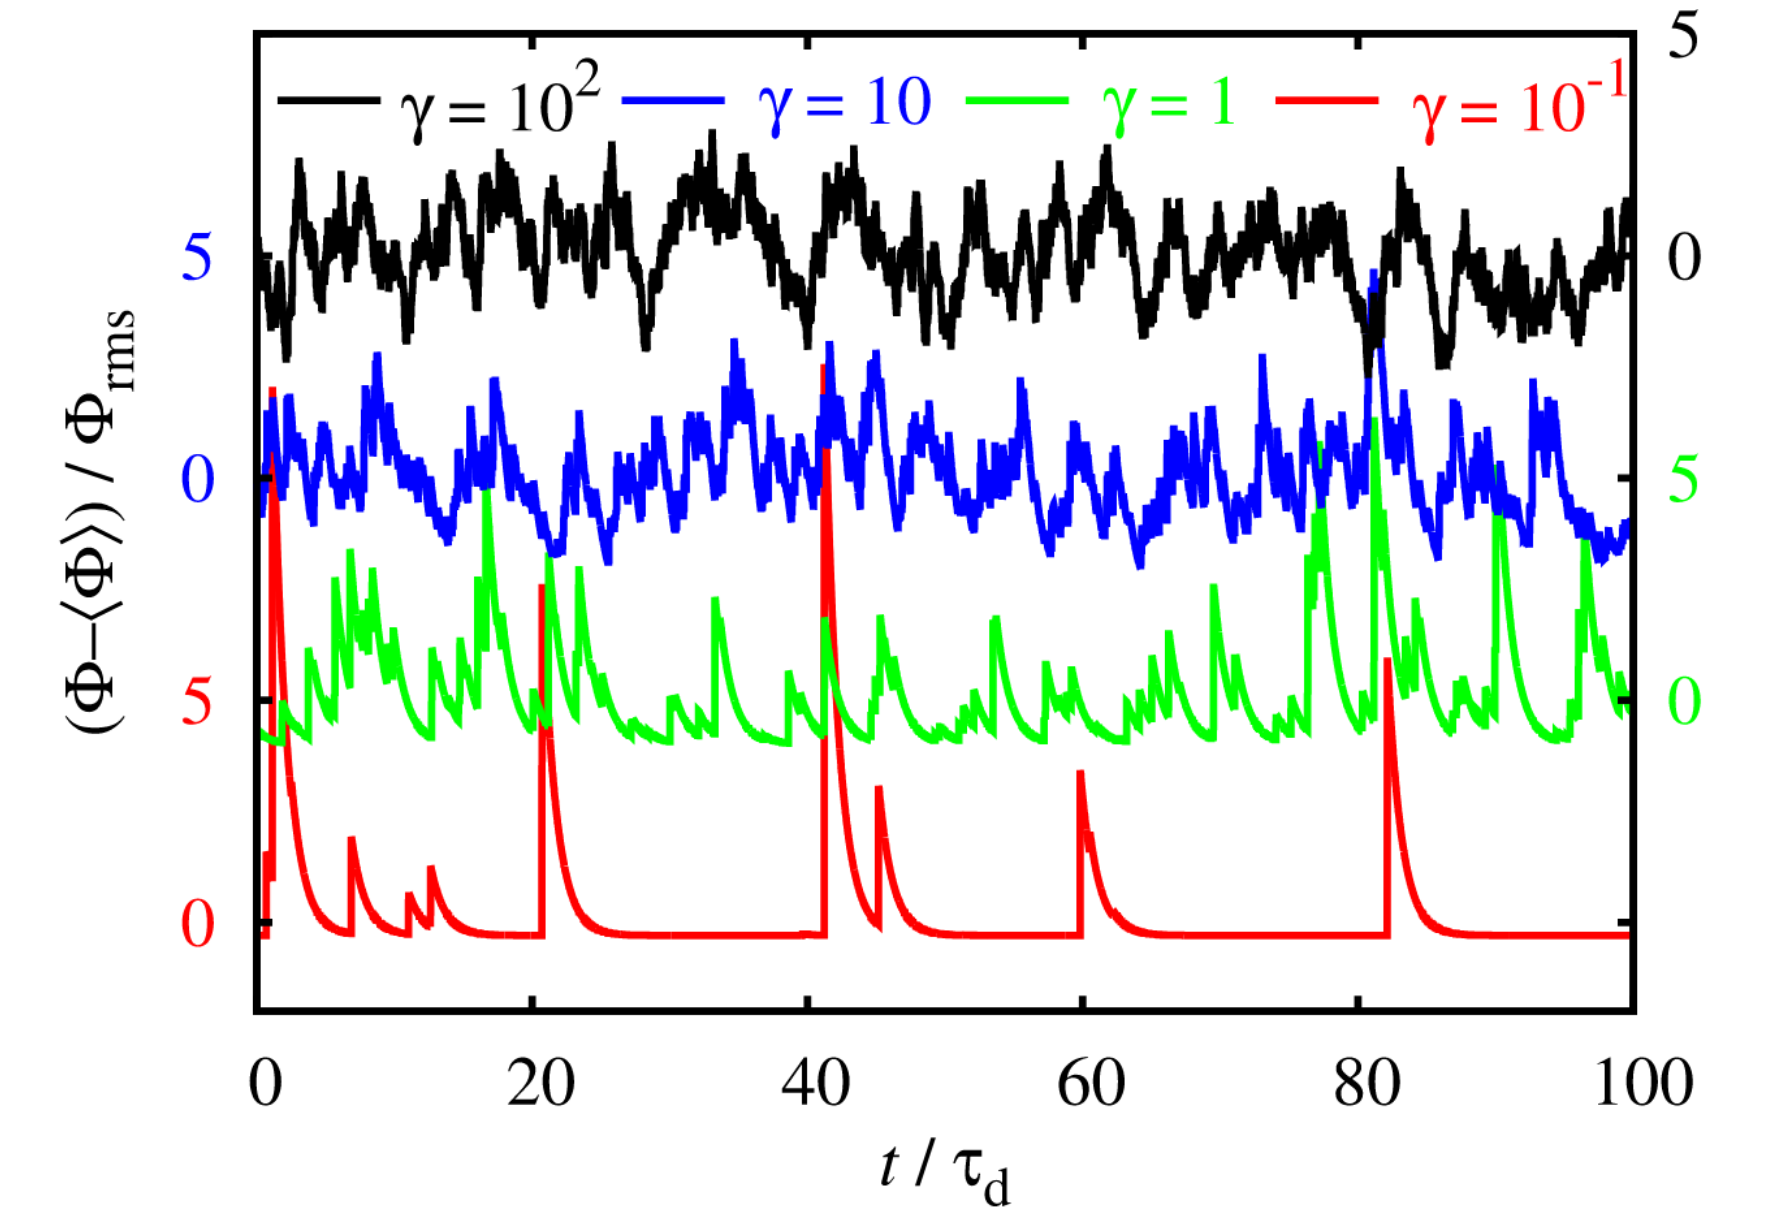
\includegraphics[width=\linewidth]{figures/garcia_realizations.png}
% 		\caption{Realizations of the FPP with one-sided exponential pulses and different intermittency parameters. Reprinted from \cite{garcia2016stochastic}, with the permission from AIP Publishing.}
% 		\label{Fig:garcia_realizations}
% 	\end{minipage}
% 	\hfill
% 	\begin{minipage}{.48\linewidth}
% 		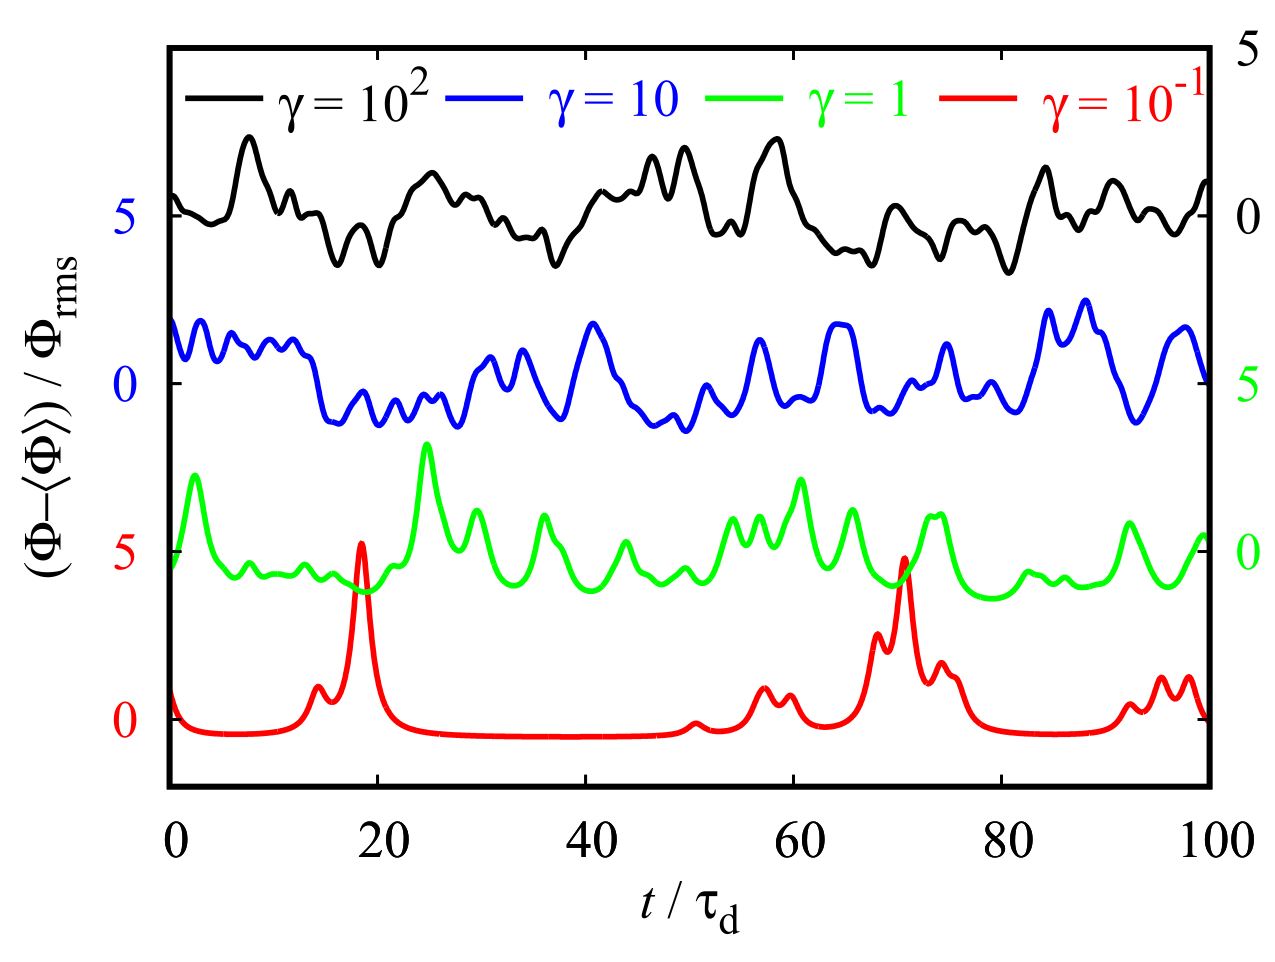
\includegraphics[width=\linewidth]{figures/garcia_lorentz.png}
% 		\caption{Realizations of the FPP with Lorentzian pulses and different intermittency parameters. Reprinted from \cite{garcia2017power}, with the permission from AIP Publishing.}
% 		\label{Fig:garcia_realizations_lorentz}
% 	\end{minipage}
% \end{figure}

% \section{Moments and PDFs}
% The four lowest order central moments of the FPP take the form 
% \begin{subequations}
% 	\begin{align}
% 		\langle\Phi\rangle  &= \gamma \langle A \rangle I_1,\\
% 		\Phi^2_\mathrm{rms} &= \gamma \langle A^2\rangle I_2,\\
% 		S_\Phi &= \frac{1}{\gamma^{1/2}}\frac{\langle A^3\rangle I_3}{\langle A^2\rangle^{3/2} I_2^{3/2} },\\
% 		F_\Phi &= 3 + \frac{1}{\gamma} \frac{\langle A^4\rangle I_4}{\langle A^2\rangle^2 I_2^2}, 
% 	\end{align}
% \end{subequations}
% where $S_\Phi$ stands for the skewness of the process and $F_\Phi$ is the kurtosis or flatness \cite{garcia2012stochastic}. The last two moments exhibit the parabolic relationship 
% \begin{equation}\label{parabolic}
% 	F_\Phi = 3 + \frac{\langle A^2\rangle \langle A^4\rangle}{\langle A^3\rangle^2}\frac{I_2 I_4}{I^2_3} S_\Phi^2.
% \end{equation}
% Inserting the expressions for the integrals of the pulse shapes for two-sided exponential and Lorentzian pulses and assuming exponentially distributed amplitudes simplifies these expressions further. For exponential pulses the expression for the relative fluctuation level becomes
% \begin{equation}
% 	\frac{\Phi_{\mathrm{rms}}}{\langle \Phi\rangle} = \gamma^{-1/2},
% \end{equation}
% and the universal parabolic relationship of \Eqref{parabolic} reduces to
% \begin{equation}
% 	F_\Phi = 3 + \frac{3}{2} S_\Phi^2,
% \end{equation} 
% which stands in good agreement with experimental measurements \cite{labit2007universal,sattin2009statistics,sattin2009parabolic}. Notably, these expressions do not depend on the pulse asymmetry parameter, $\lambda$. 

% The PDF of the process with exponential pulses is given by a Gamma distribution with shape parameter $\gamma$ and scale parameter $\langle A \rangle$ \cite{theodorsen2018probability},

% \begin{equation}
% 	P_{\Phi,\phi}(\Phi) = \frac{\Phi^{\gamma-1}}{\langle A\rangle^\gamma \Gamma(\gamma)}\mathrm{exp}\left(-\frac{\Phi}{\langle A\rangle}\right).
% \end{equation}
% Typically, the realization of the process is normalized to have zero mean and unit standard deviation,
% \begin{equation}\label{norm}
% 	\widetilde{\Phi} = \frac{\Phi - \langle\Phi\rangle}{\Phi_{\mathrm{rms}}},
% \end{equation}
% with the according PDF \cite{theodorsen2018probability},
% \begin{equation}
% 	P_{\widetilde{\Phi},\phi}(\widetilde{\Phi}) = \frac{\gamma^{\gamma/2}}{\Gamma(\gamma)}\left(\widetilde{\Phi} + \gamma^{1/2} \right)^{\gamma-1}\mathrm{exp}\left(-\gamma^{1/2}\widetilde{\Phi} - \gamma\right).
% \end{equation}
% This expression is used as a fit in \Figref{Fig:theodorsen_pdf}. For an FPP of Lorentzian pulses no closed expressions for its PDF is known. However, it can be derived by taking the inverse Fourier transform of its corresponding characteristic function resulting in \cite{garcia2018lorentz}
% \begin{equation}
% 	\begin{split}
% 	P_{\widetilde{\Phi},\psi}(\widetilde{\Phi}) = \left(\frac{\pi}{\gamma}\right)^{1/2}\int_{0}^{\infty}\textrm{d}w\,\mathrm{exp}\left(-\frac{\gamma\pi w\, \mathrm{sin}\left(1/2\, \mathrm{arctan}\, w\right)}{(1+w^2)^{1/4}}\right)\\
% 	\times \mathrm{cos}\left(\pi\gamma w + \sqrt{\pi\gamma}\widetilde{\Phi}w-\frac{\gamma\pi w\, \mathrm{cos}\left(1/2\, \mathrm{arctan}\, w\right)}{(1+w^2)^{1/4}}\right).
% 	\end{split}
% \end{equation}
% For both exponential and Lorentzian pulses the PDF of the processes are characterized by the intermittency parameter. The PDFs are shown for a range of different $\gamma$ in \Figref{Fig:garcia_pdf} and \Figref{Fig:garcia_pdf_lorentz}. The PDFs are unimodal for all values of $\gamma$ and have an exponential tail towards large fluctuation amplitudes for small values of $\gamma$. In the opposite limit, the PDFs approach a normal distribution with vanishing mean and unit standard deviation for $\widetilde{\Phi}$.

% \begin{figure}
% 	\centering
% 	\begin{minipage}{.48\linewidth}
% 		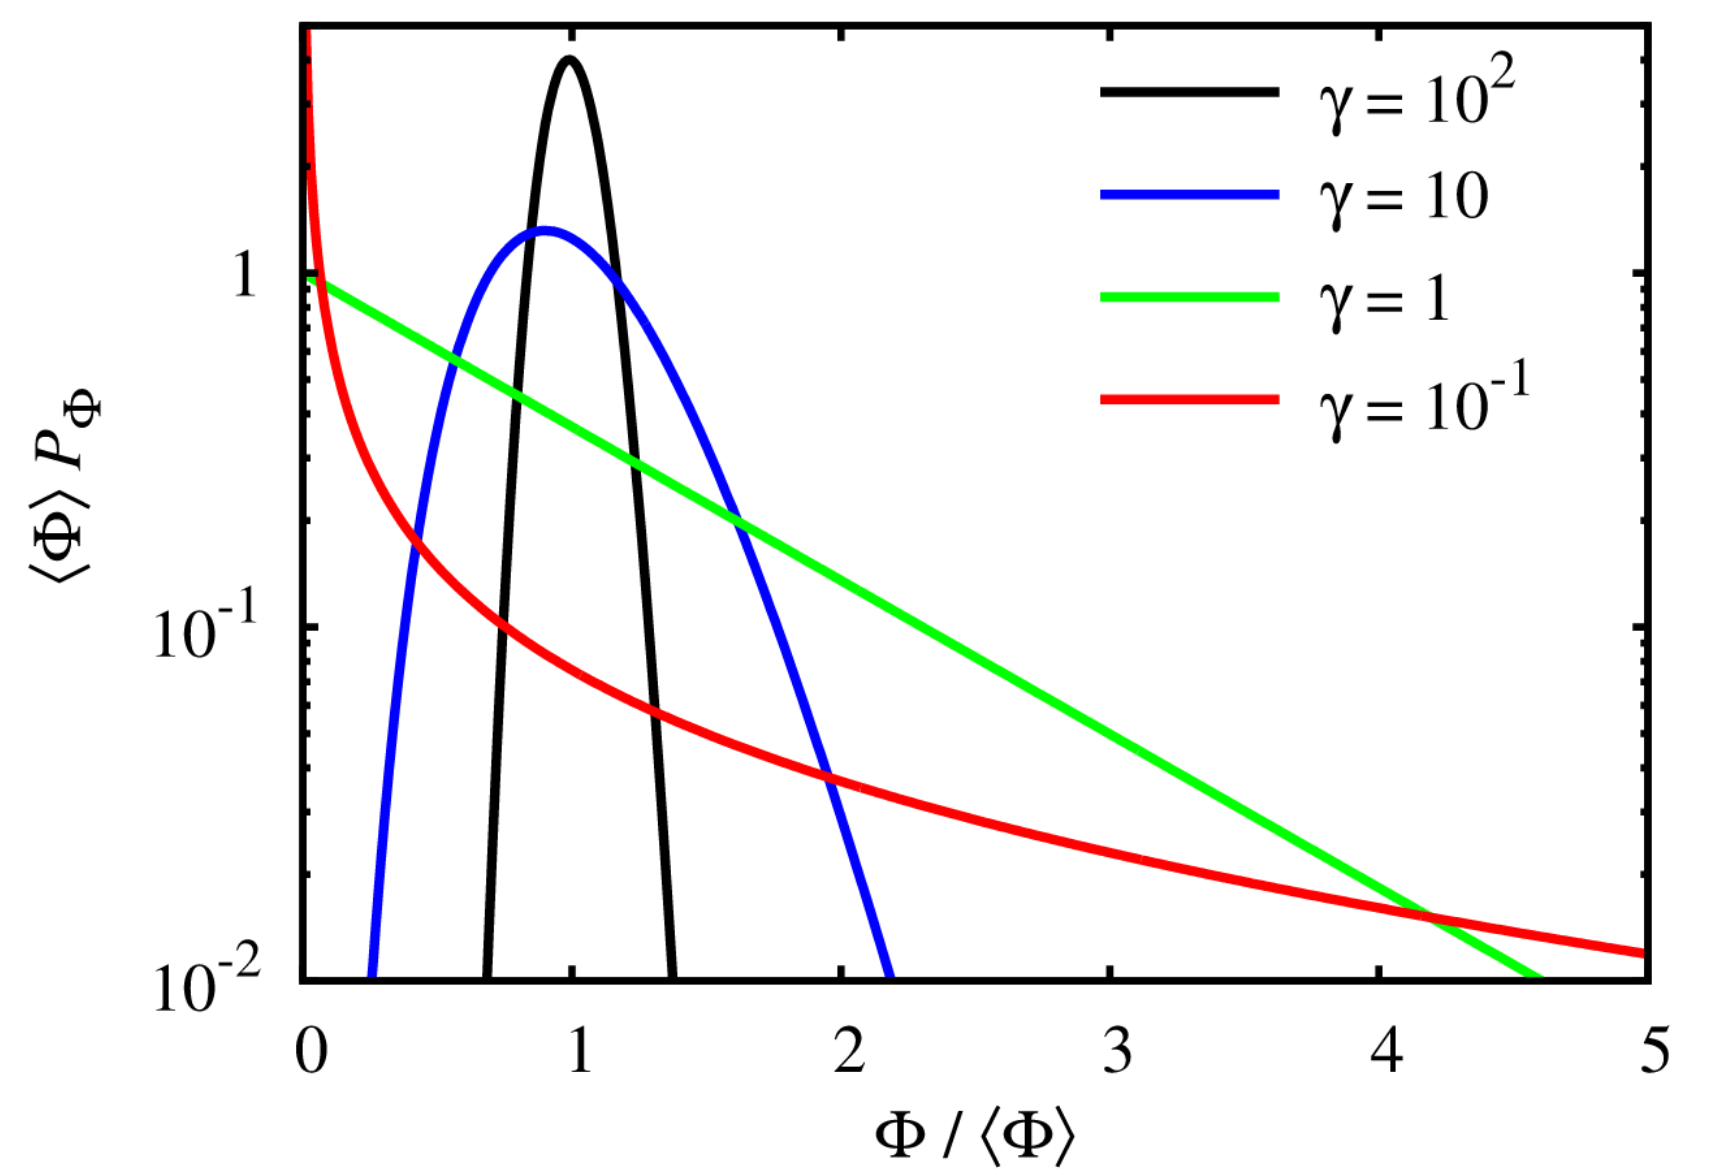
\includegraphics[width=\linewidth]{figures/garcia_pdf.png}
% 		\caption{PDFs of a FPP with exponential pulses with different intermittency parameters $\gamma$. Reprinted from \cite{garcia2016stochastic}, with the permission from AIP Publishing.}
% 		\label{Fig:garcia_pdf}
% 	\end{minipage}
% 	\hfill
% 	\begin{minipage}{.48\linewidth}
% 		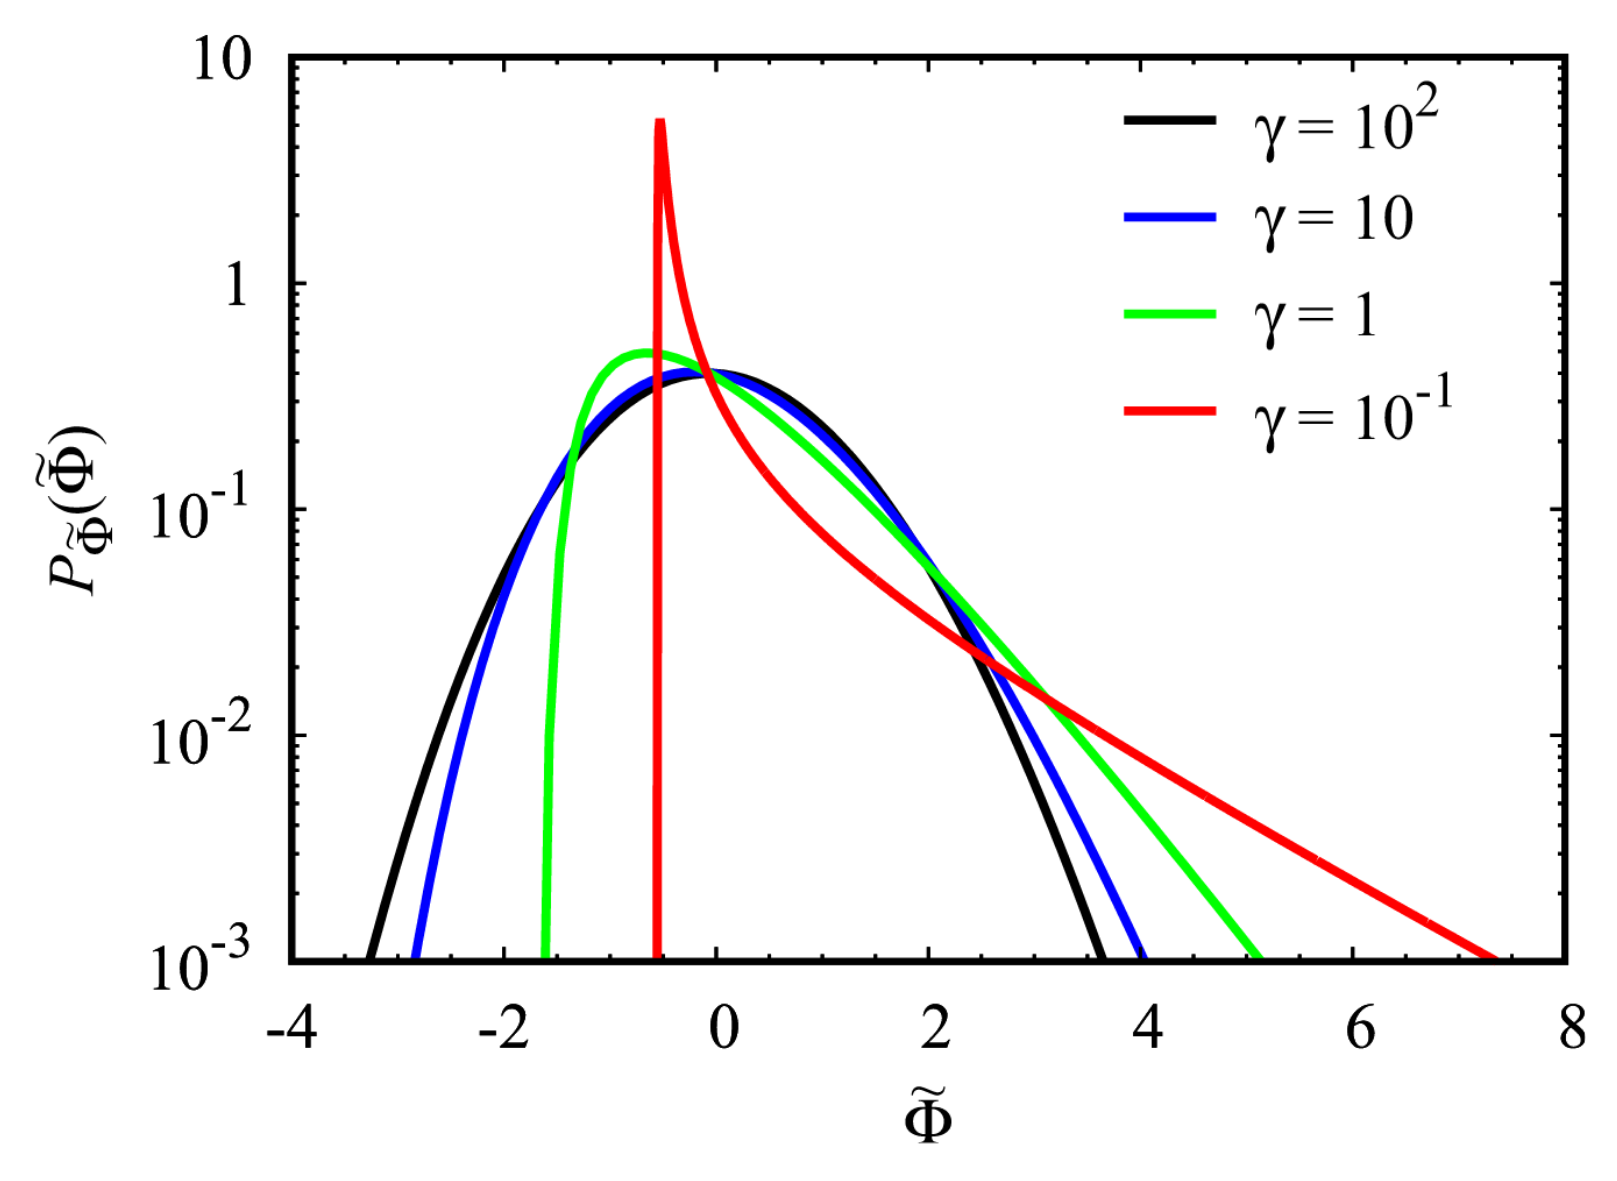
\includegraphics[width=\linewidth]{figures/garcia_pdf_lorentz.png}
% 		\caption{PDFs of a normalized FPP with Lorentzian pulses with different intermittency parameters $\gamma$. Reprinted from \cite{garcia2018lorentz}, with the permission from AIP Publishing.}
% 		\label{Fig:garcia_pdf_lorentz}
% 	\end{minipage}
% \end{figure}
% \section{Second order statistics}

% In order to calculate the second order moments, namely the power spectral density (PSD) and the Auto-correlation function (ACF), we consider the FPP as a convolution of a pulse train $f_K$ and a pulse shape $\phi$. The Fourier transform of the FPP is given by the product of the Fourier transform of $f_K$ and $\phi$. The power spectrum of $\Phi$ can therefore be expressed as the product of the power spectrum of $f_K$ and $\phi$. The power spectrum of $f_K$ is flat due to the uncorrelated delta pulses, so that the frequency dependence of the spectrum of $\Phi$ is only dependent on $\phi$. The ACF is given by the Fourier transform of the PSD. For two-sided exponential pulses the PSD of an FPP normalized according to \Eqref{norm}, takes the form \cite{garcia2017auto}
% \begin{equation}
% 	\Omega_{\widetilde{\Phi},\phi}(\omega;\lambda) = \frac{2 \tau_\mathrm{d}}{[1+(1-\lambda)^2\tau_\mathrm{d}^2\omega^2][1+\lambda^2\tau_\mathrm{d}^2\omega^2]},
% \end{equation}
% with the according ACF
% \begin{equation}
% 	R_{\widetilde{\Phi},\phi}(r;\lambda) = \frac{1}{1-2\lambda}\left[\left(1-\lambda\right)\mathrm{exp}\left(-\frac{|r|}{(1-\lambda)\tau_\mathrm{d}}\right) -\lambda\,\mathrm{exp}\left(-\frac{|r|}{\lambda\tau_\mathrm{d}}\right)\right].
% \end{equation}
% The ACF and PSD are displayed for a range of $\gamma$-values in \Figsref{Fig:garcia_acf} and \ref{Fig:garcia_psd}.
% \begin{figure}
% 	\centering
% 	\begin{minipage}{.48\linewidth}
% 		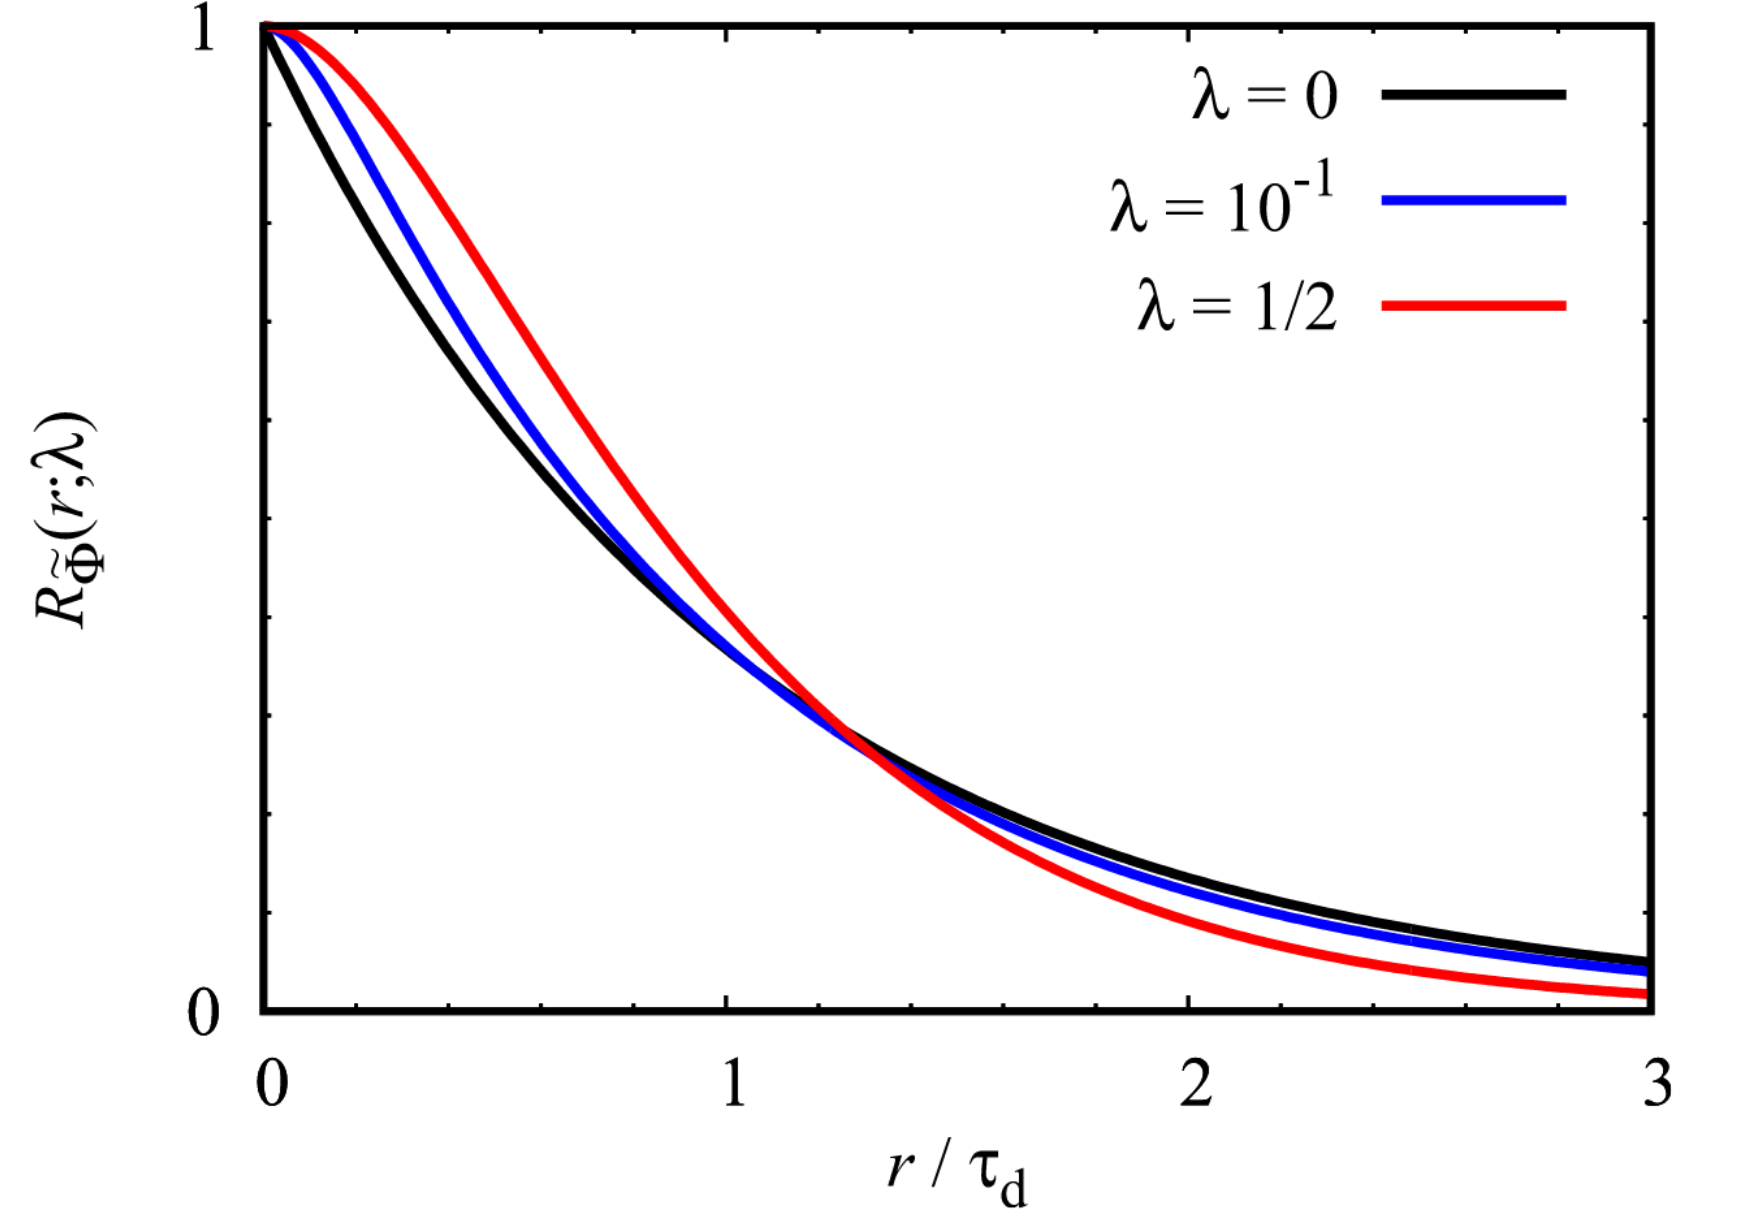
\includegraphics[width=\linewidth]{figures/garcia_acf.png}
% 		\caption{Auto-correlation function of a normalized FPP consisting of two-sided exponential pulses with different asymmetry parameters $\lambda$. Reprinted from \cite{garcia2017auto}, with the permission from AIP Publishing.}
% 		\label{Fig:garcia_acf}
% 	\end{minipage}
% 	\hfill
% 	\begin{minipage}{.48\linewidth}
% 		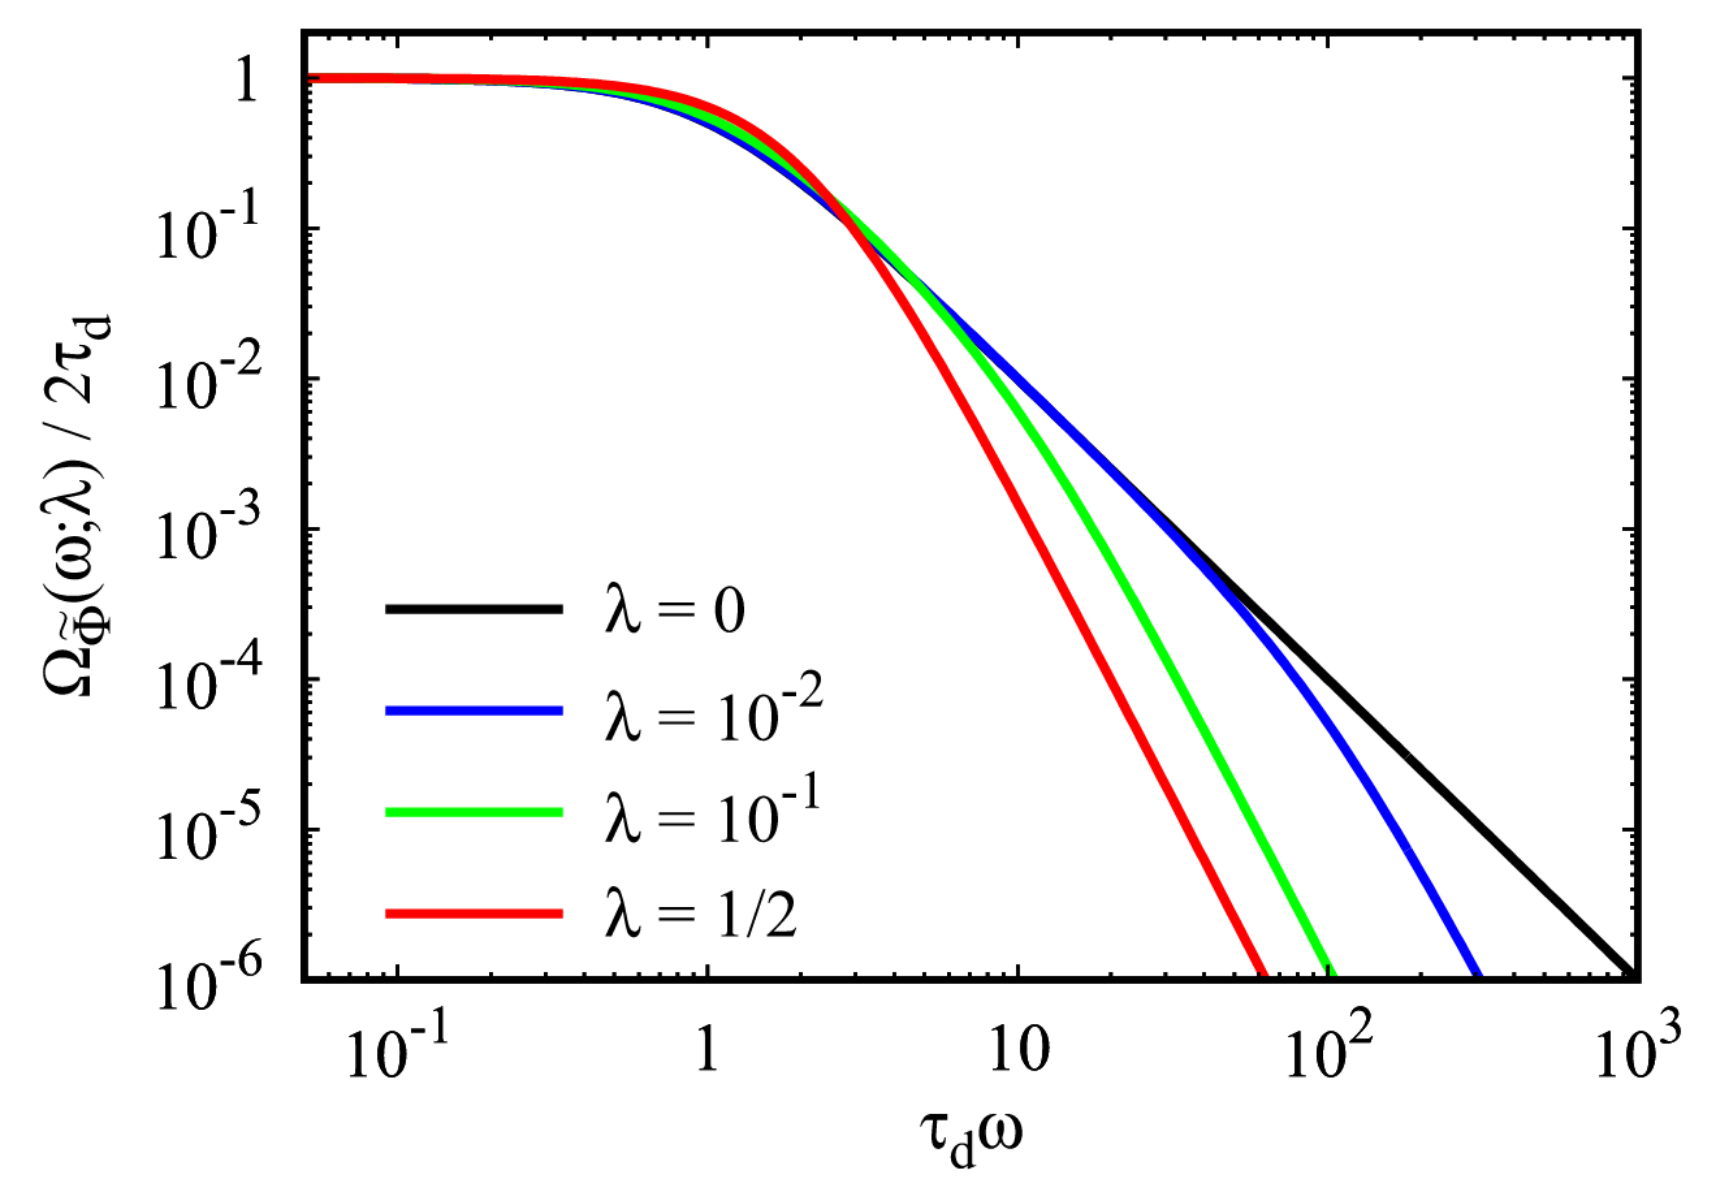
\includegraphics[width=\linewidth]{figures/garcia_psd.png}
% 		\caption{Power spectral density of a normalized FPP consisting of two-sided exponential pulses with different asymmetry parameters $\lambda$. Reprinted from \cite{garcia2017auto}, with the permission from AIP Publishing.}
% 		\label{Fig:garcia_psd}
% 	\end{minipage}
% \end{figure}
% In contrast to the PDFs, the second order statistics are independent of $\gamma$ but change for different $\lambda$. In the limits of a one-sided exponential pulse, the ACF is purely exponential and the PSD is Lorentzian shaped. For $\lambda$ close to zero or 1, the spectrum has an intermediate range where the spectrum falls with $\omega^{-2}$ before it falls with $\omega^{-4}$ in the high frequency limit. This expression is in excellent agreement with the experimental measurements shown in \Figref{Fig:theodorsen_psd} with $\lambda=0.1$. 

% For Lorentzian pulses the PSD of a normalized FPP takes an exponential form \cite{garcia2018skewed}
% \begin{equation}
% 	\Omega_{\widetilde{\Phi},\psi}(\omega) = 2\pi\tau_\mathrm{d}\, \mathrm{exp}\left(-2\tau_\mathrm{d}|\omega|\right),
% \end{equation}
% and the ACF is Lorentzian shaped,
% \begin{equation}
% 	R_{\widetilde{\Phi},\psi}(r) = \frac{4}{4+(r/\tau_\mathrm{d})^2}.
% \end{equation}
% These expressions can be generalized to skewed Lorentzian pulses, however no closed expressions are known. An alternative formulation is presented in \cite{garcia2018skewed}.

% \section{Excess time statistics}
% Expressions for excess time statistics, specifically the rate of level crossings above a given threshold and the average time spent above this threshold, can be derived for an FPP. In the context of fluctuations in the SOL of fusion experiments, these quantities are crucial considering the energy of incoming particles to the vessel walls and the energy threshold of physical sputtering. The number of sputtered particles per incoming particle is specified by the modified Bohdansky yield function \cite{marandet2016assessment}. The mean yield as a function of energy of an incoming deuterium particle on a tungsten wall is plotted for a range of relative fluctuation levels in \Figref{Fig:theodorsen_yield}. For constant energy, no sputtering occurs beneath 200 eV. For realistic scenarios of $E_\mathrm{rms}/\langle E\rangle > 0$ sputtering already occurs at significantly lower mean energies. An accurate description of excess time statistics is therefore of importance for fusion experiments. 

% For an FPP the number of level crossings is given by Rice's formula \cite{rice1945mathematical}
% \begin{equation}
% 	X(\Phi) = T\int_{0}^{\infty} \mathrm{d}\dot{\Phi}\, \dot{\Phi}P_{\Phi,\dot{\Phi}}\left(\Phi,\dot{\Phi}\right).
% \end{equation}
% Here $\dot{\Phi}$ stands for the derivative of the process $\Phi$ and $P_{\Phi,\dot{\Phi}}\left(\Phi,\dot{\Phi}\right)$ for the joint PDF between $\Phi$ and $\dot{\Phi}$. This formulation requires the process to be differentiable, hence an FPP consisting of one-sided exponential pulses cannot be considered this way. For two-sided exponential pulses with $\lambda \in (0,1)$ the rate of up-crossings is given by \cite{theodorsen2018level}
% \begin{equation}\label{rate}
% 	\frac{\tau_\mathrm{d}}{T}X(\Phi) = \frac{\lambda^{\gamma\lambda-1}(1-\lambda)^{\gamma(1-\lambda)-1}}{\gamma\Gamma(\gamma\lambda)\Gamma(\gamma(1-\lambda))}\left(\frac{\gamma\Phi}{\langle\Phi\rangle}\right)^\gamma\mathrm{exp}\left(-\frac{\gamma\Phi}{\langle\Phi\rangle}\right).
% \end{equation}
% For this expression, the limit $\lambda\rightarrow0$ exists. \Eqref{rate} is plotted for exponential pulses with $\lambda=0$ and $\lambda=1/2$ and a range of $\gamma$-values in \Figref{Fig:theodorsen_avtime}. From this, the PDF of time as well as mass above a given threshold can be determined analytically for the limits $\gamma\rightarrow 0$ and $\gamma\rightarrow \infty$  and numerically with Monte Carlo simulations for general $\gamma$ \cite{theodorsen2018level}. 
% \begin{figure}
% 	\centering
% 	\begin{minipage}{.48\linewidth}
% 		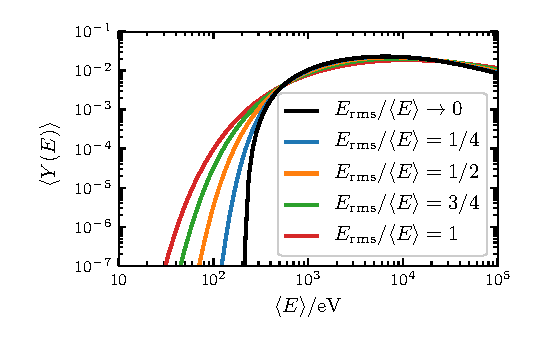
\includegraphics[width=\linewidth]{figures/yield_fun_mE_W.eps}
% 		\caption{Mean yield  function for a range of relative fluctuation levels. Image courtesy of A. Theodorsen \cite{theodorsen2018statistical}.}
% 		\label{Fig:theodorsen_yield}
% 	\end{minipage}
% 	\hfill
% 	\begin{minipage}{.48\linewidth}
% 		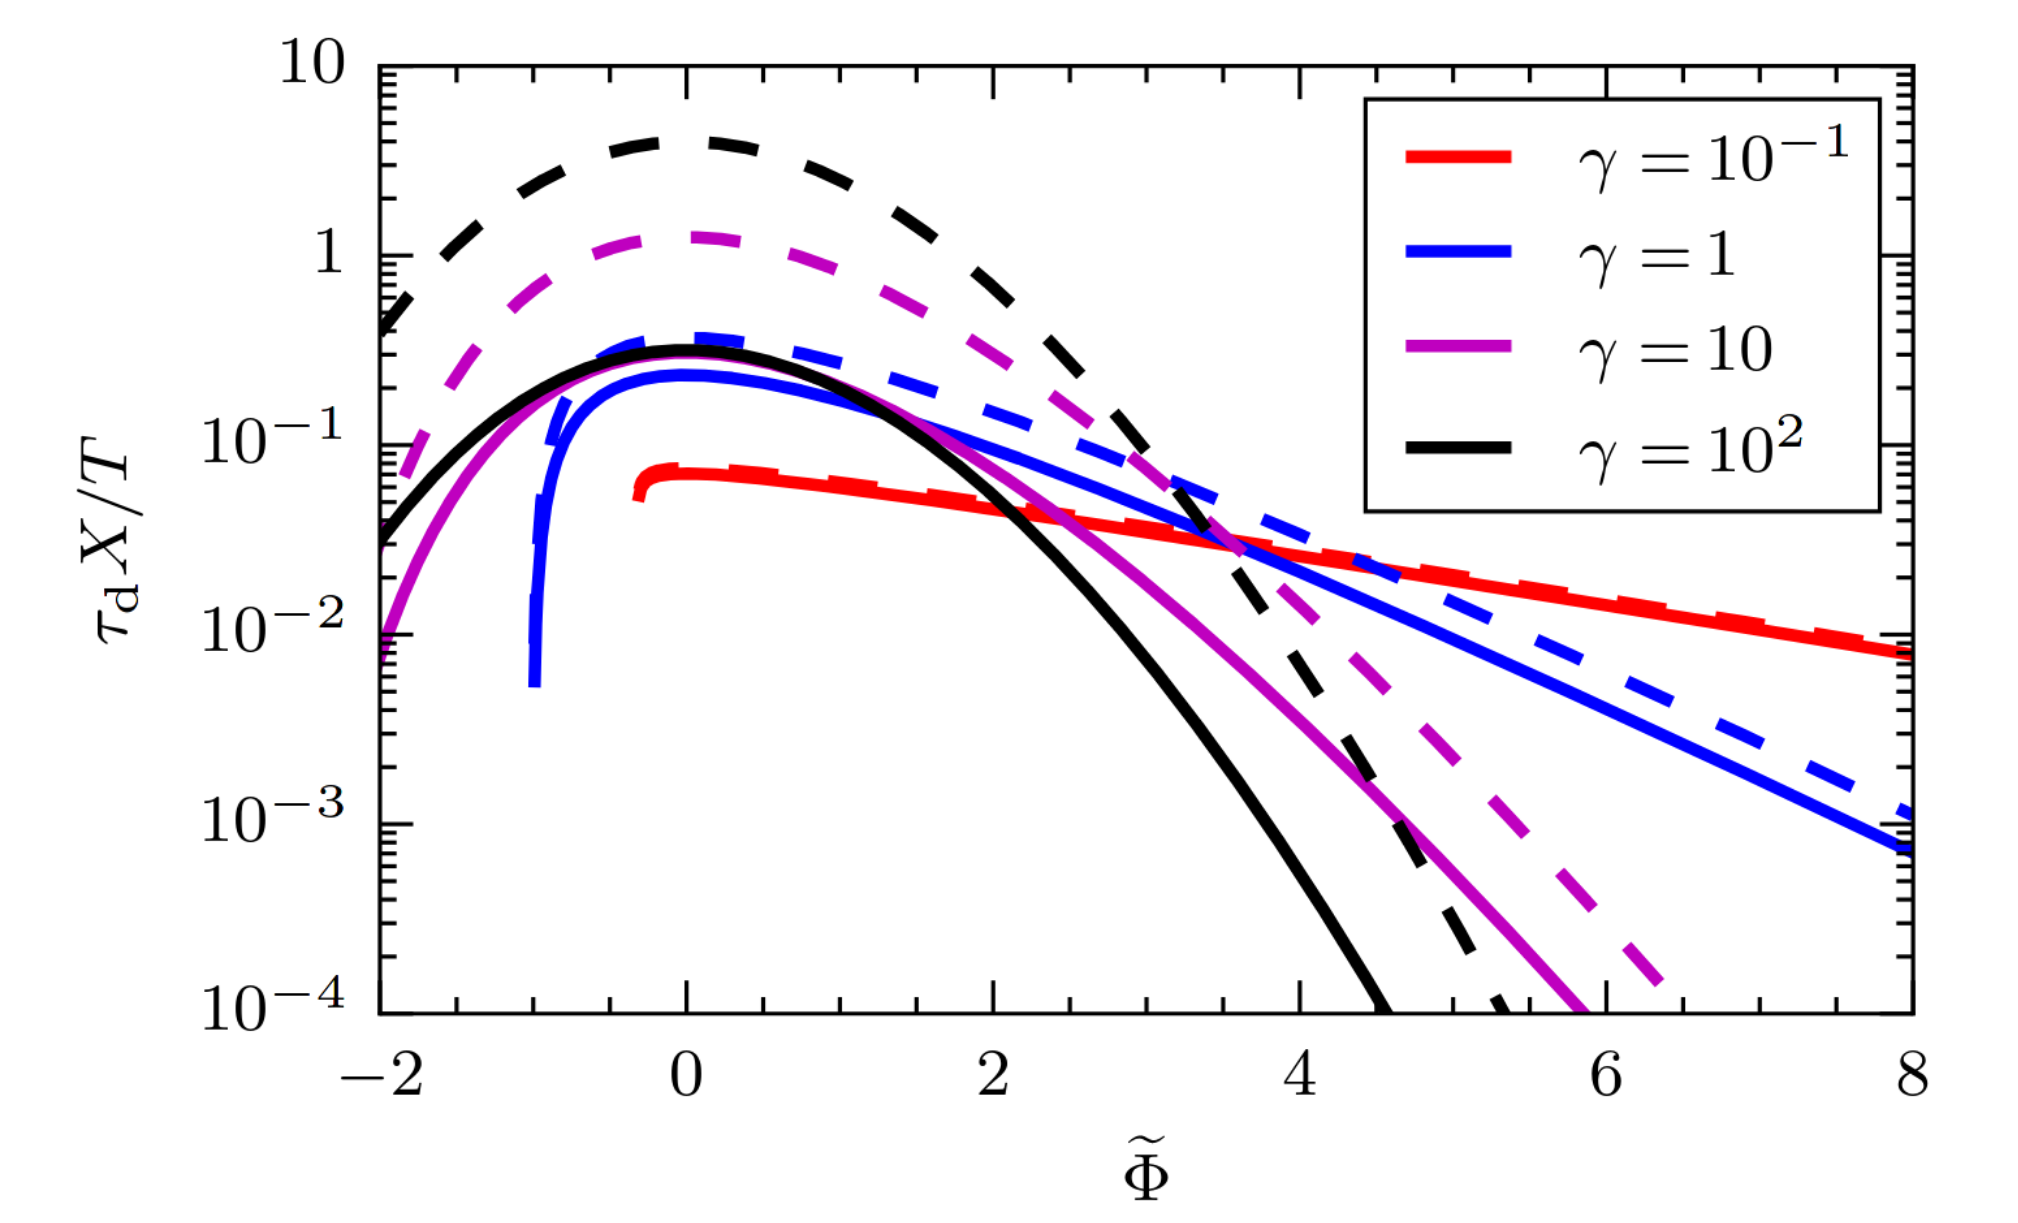
\includegraphics[width=\linewidth]{figures/theodorsen_rate.png}
% 		\caption{Rate of up-crossings for a FPP consisting of exponential pulses with $\lambda=0$ (dashed line) and $\lambda=1/2$ (full line) for various $\gamma$-values. Reprinted figure with permission from \cite{theodorsen2018level}. Copyright (2018) by the American Physical Society.}
% 		\label{Fig:theodorsen_avtime}
% 	\end{minipage}
% \end{figure}

% At the time of writing this thesis, excess time statistics of an FPP consisting of Lorentzian pulses have not been investigated.

% \section{Density profiles}\label{n_prof}
% The FPP can be extended to include a spatial variable $x$, resulting in a model of advecting single pulses and corresponding profiles. In the following, this model is discussed in the context of filament motion in SOL plasmas. The presented notation is consistent with \cite{garcia2016stochastic}. Alternative formulations based on a Lagrangian approach to filament dynamics result in equivalent expressions \cite{militello2016scrape,militello2016relation,walkden2017interpretation,militello2018two}.

% The model is given by a superposition of pulses 
% \begin{equation}
% 	\Phi_K(x,t) = \sum_{k=1}^{K} \phi_k(x,t).
% \end{equation}
% In contrast to previous sections $\phi_k$ is compounded by both amplitude and pulse shape. For simplicity, we keep $K$ constant in the following derivation. The evolution of individual pulses, neglecting pulse interaction, is given by the modified advection equation,
% \begin{equation}\label{phi_equation}
% 	\frac{\partial \phi_k}{\partial t} + v_\perp\frac{\partial \phi_k}{\partial x} + \frac{\phi_k}{\tau_\parallel} = 0,
% \end{equation}
% with $v_\perp$ as the radial velocity and $\tau_\parallel$ representing the parallel transit time, describing parallel losses along the magnetic field. Note, that we assume $v_\perp$ and $\tau_\parallel$ to be constant for all filaments. Following \Eqref{phi_equation}, individual pulses can be written as the product of their amplitude and pulse shape, $	\phi_k(x,t) = A_k(t)\varphi_k(x-x_k-v_k t)$ with $x_k$ as the position of the pulse at $t=0$. The individual amplitudes are assumed to satisfy the expression 
% \begin{equation}
% 	\frac{\mathrm{d}A_k}{\mathrm{d}t} = -\frac{A_k}{\tau_\parallel}.
% \end{equation}
% The solution for this amplitude equation can be expressed by introducing the initial amplitude $A_{0k}$ resulting in
% \begin{equation}
% 	A_k(t) = A_{0k}\,\mathrm{exp}\left(-\frac{t+x_k/v_\perp}{\tau_\parallel}\right),
% \end{equation}
% with the pulse $k$ being located at $x=0$ at time $-x_k/v_\perp$. We further assume the pulse shape to take the form of an exponential function,
% \begin{equation}
% 	\varphi_k(x) = \Theta\left(-\frac{x}{l_\perp}\right)\mathrm{exp}\left(\frac{x}{l_\perp}\right),
% \end{equation}
% where $\Theta$ is the Heaviside function and $l_\perp$ is the radial size of the pulse. Note, that this pulse shape is consistent with the findings shown in \Figref{Fig:garcia_1}. We now consider the signal at a reference position $\xi$. At the reference time $t_k = (\xi - x_k)/v_\perp$ for pulse $k$ at position $\xi$, the process takes the form
% \begin{equation}
% 	\Phi_K(\xi, t) = \sum_{k=1}^{K}A_{0k}\,\mathrm{exp}\left(-\frac{\xi}{v_\perp \tau_\parallel}\right)\Theta\left(\frac{t-t_k}{\tau_\perp}\right)\exp\left(-\frac{t-t_k}{\tau_\mathrm{d}}\right),
% \end{equation}
% with $\tau_\perp = l_\perp/v_\perp$ and the pulse duration given by the harmonic mean of the perpendicular and parallel transit time $\tau_\mathrm{d} = \tau_\parallel\tau_\perp/(\tau_\parallel+\tau_\perp)$. By averaging over uniformly distributed pulse arrivals, the resulting radial profile takes the exponential form
% \begin{equation}
% 	\langle\Phi\rangle(\xi) = \frac{\tau_\mathrm{d}}{\tau_w}\langle A_0\rangle\mathrm{exp}\left(-\frac{\xi}{v_\perp\tau_\parallel}\right).
% \end{equation}
% The resulting scale length of the profile is governed by the radial velocity of the filaments and the parallel transit time. Multiple realizations at individual points in time and the corresponding mean profile are shown in \Figref{Fig:militello}. 

% The application of this model exhibits numerous limitations. The assumption of constant radial velocities and pulse size is an overly simplified description for filament transport in the SOL. In addition, the assumption of radially constant $\tau_w$ and therefore radially constant $\gamma$ does not hold in experimental observations. Interactions between individual filaments and two-dimensional motion are also not considered. However, this mathematical model still provides valuable insight in the relation between individual filaments and radial profiles in the SOL and can serve as a framework to relate isolated blob and filament studies to turbulence simulations and experimental measurements. 

% \begin{figure}[t]
% 	\centering
% 	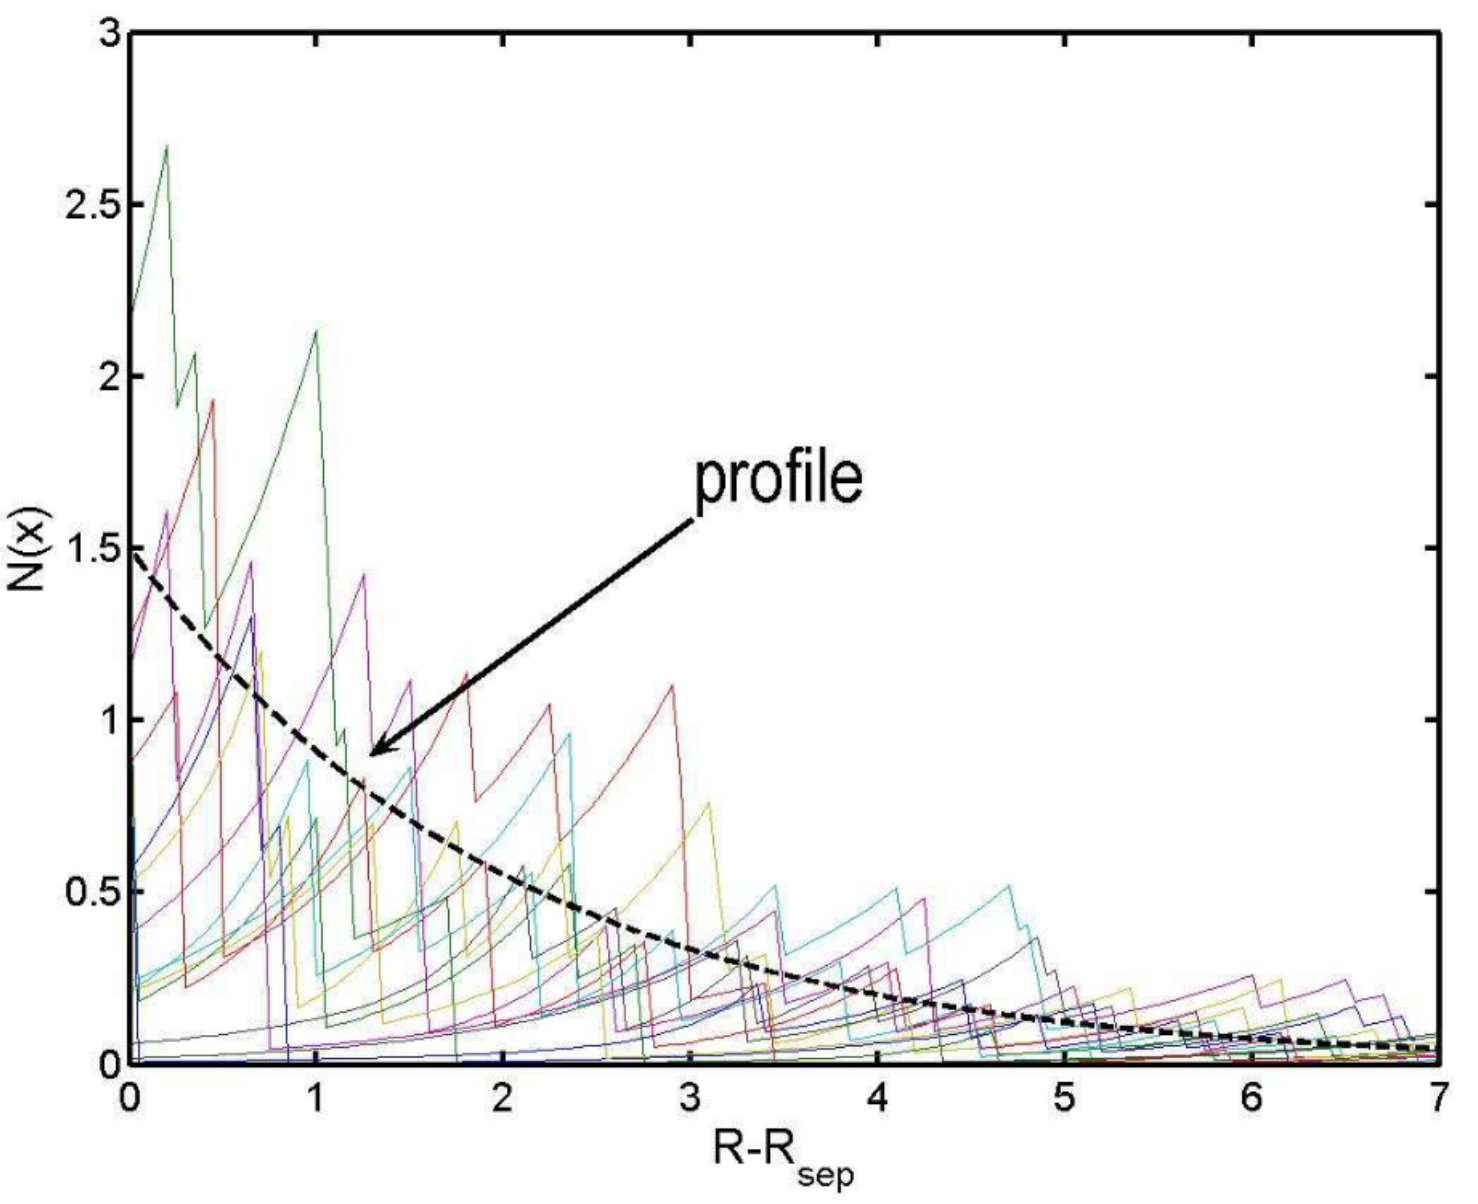
\includegraphics[width=9cm]{figures/militello_profile.png}
% 	\caption{Radial exponential density profile (black dashed line) illustrated as the mean of individual density realizations (colored lines) given by a superposition of individual exponentially shaped pulses. Image courtesy of F. Militello \cite{militello_profiles}.}
% 	\label{Fig:militello}
% \end{figure}
% \section{Deconvolution method}
% Since the FPP can be expressed as a convolution of a pulse function $\phi$ and a forcing, consisting of delta-function pulses $f_K$, shown in \Eqref{conv}, one can attempt to estimate the forcing if the pulse shape is known \cite{theodorsen2018universality, decristoforo2020intermittent, kube2020comparison}. For a given forcing, one can determine the pulse amplitudes $\{ A_k \}_{k=1}^K$ and arrival times $\{ t_k \}_{k=1}^K$ directly. This method has the advantage of capturing pulses of all sizes, not only events above a certain threshold as is the case for conditional averaging. Additionally, the problem of pulse overlap is less severe. In order to estimate the forcing, a modified Richardson-Lucy deconvolution algorithm can be used \cite{richardson1972bayesian,lucy1974iterative}. The algorithm is initialized with a first guess for the forcing $f_K^{(1)}$. This value is iteratively updated with the $n$-th iteration given by
% \begin{equation}
% 	f_K^{(n+1)} = f_K^{(n)} \frac{D*\widehat{\phi}}{f_K^{(n)}*\phi*\widehat{\phi}}.
% \end{equation}
% Here, $\widehat{\phi}(t) = \phi(-t)$ and $D$ denotes the investigated time series. This algorithm converges to the least squares solution \cite{dell2007model}. The initial guess for the forcing matters little as it only determines the number of iterations required until the algorithm converges. 

% This deconvolution algorithm thereby provides a versatile tool to analyze time series of SOL fluctuations in experiments and simulations, as it can provide clear results even for relatively short time series.   


